\documentclass[11pt,a4paper]{article}
\usepackage[utf8]{inputenc}
\usepackage{graphicx}
\usepackage{amsmath}
\usepackage{listings}
\usepackage{xcolor}
\usepackage{hyperref}
\usepackage{tikz}
\usepackage{pgfplots}
\pgfplotsset{compat=1.18}

\definecolor{codegreen}{rgb}{0,0.6,0}
\definecolor{codegray}{rgb}{0.5,0.5,0.5}
\definecolor{codepurple}{rgb}{0.58,0,0.82}
\definecolor{backcolour}{rgb}{0.95,0.95,0.92}

\lstdefinestyle{mystyle}{
    backgroundcolor=\color{backcolour},   
    commentstyle=\color{codegreen},
    keywordstyle=\color{magenta},
    numberstyle=\tiny\color{codegray},
    stringstyle=\color{codepurple},
    basicstyle=\ttfamily\footnotesize,
    breakatwhitespace=false,         
    breaklines=true,                 
    captionpos=b,                    
    keepspaces=true,                 
    numbers=left,                    
    numbersep=5pt,                  
    showspaces=false,                
    showstringspaces=false,
    showtabs=false,                  
    tabsize=2
}

\lstset{style=mystyle}

\title{\textbf{System Introduction Lab 2: Multi-threaded Matrix Multiplication}}
\author{WangLiming \& PanChangxun}
\date{April, 2025}

\begin{document}

\maketitle

\section{Introduction}
This report presents the implementation and analysis of a multi-threaded matrix multiplication system. Building upon Lab 1's single-threaded implementation, this lab extends the functionality to utilize multiple cores on the Raspberry Pi through concurrent execution. The lab is structured into four tasks, each building upon the previous one to achieve the final goal of a high-performance, multi-threaded matrix multiplication system.

\section{Task 1: Implementation of the Task Queue}

\subsection{Design and Implementation}
For Task 1, we implemented a thread-safe queue that supports multiple producers and consumers. The queue implementation uses a circular buffer design pattern to efficiently store and retrieve matrix multiplication tasks.

Key components of the implementation include:
\begin{itemize}
    \item A closed flag to indicate when no more items will be added
    \item Synchronization primitives:
    \begin{itemize}
        \item \texttt{pthread\_mutex\_t mutex} for mutual exclusion
        \item \texttt{pthread\_cond\_t not\_empty} for consumers waiting on data
        \item \texttt{pthread\_cond\_t not\_full} for producers waiting on space
    \end{itemize}
\end{itemize}

To avoid busy waiting, we used condition variables that allow threads to sleep until the condition they're waiting for is satisfied. This approach is both CPU-efficient and responsive to changes in the queue state. The details of the queue implementation is in \texttt{queue.c}.

\subsection{Thread Model}
The thread model consists of:
\begin{itemize}
    \item One producer thread (scheduler) that creates tasks and adds them to the queue
    \item Multiple consumer threads (workers) that retrieve tasks and process them
\end{itemize}

The synchronization between threads was implemented through the following approach:
\begin{itemize}
    \item Producers wait on \texttt{not\_full} when the queue is full
    \item Consumers wait on \texttt{not\_empty} when the queue is empty
    \item Mutex locks ensure atomic operations on the queue
    \item A separate mutex for stdout prevents interleaved output
\end{itemize}

\subsection{Key Challenges and Solutions}
\begin{itemize}
    \item \textbf{Race Conditions}: Solved by consistently locking the mutex before any queue operations
    \item \textbf{Deadlocks}: Avoided by careful lock acquisition and release ordering
    \item \textbf{Spurious Wakeups}: Handled by using while loops for condition variable waits
    \item \textbf{Queue Closure}: Properly signaling all waiting threads upon queue closure
\end{itemize}

The implementation successfully passed all test cases in the \texttt{task1\_queue\_check} and produced correct, non-interleaved output for various values of \texttt{TASK1\_TASKS\_NUM} and \texttt{MAX\_QUEUE\_LEN}.

\section{Task 2: Adding Worker Code}

\subsection{Implementation}
In Task 2, we extended the queue from Task 1 to perform actual matrix multiplication operations. The implementation includes:

\begin{itemize}
    \item A scheduler thread that reads matrix data from \texttt{task2.txt}
    \item Worker threads that compute matrix multiplications
    \item Thread-safe output using mutex locks
\end{itemize}

\subsection{Performance Analysis}
We tested different numbers of worker threads to analyze the performance impact. The optimal number of worker threads was found to be 4, which aligns with the number of cores available on the Raspberry Pi.

\begin{figure}[!htb]
\centering
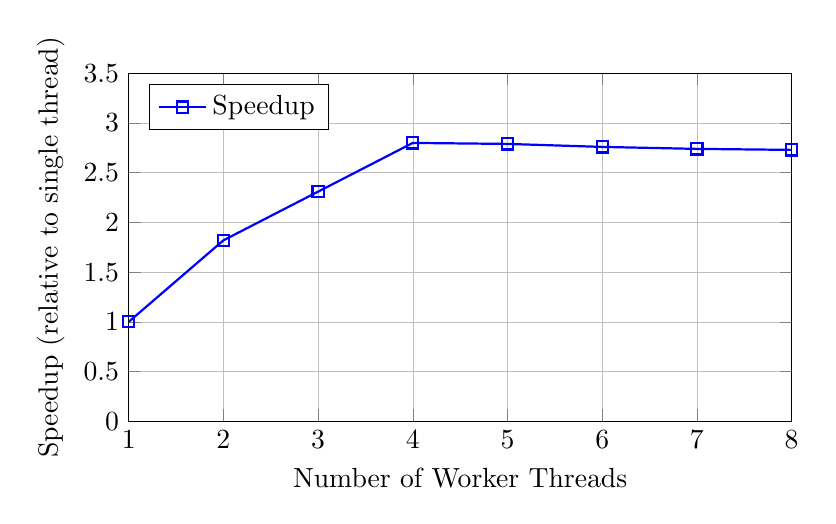
\begin{tikzpicture}
\begin{axis}[
    width=10cm,
    height=6cm,
    xlabel={Number of Worker Threads},
    ylabel={Speedup (relative to single thread)},
    xmin=1, xmax=8,
    ymin=0, ymax=3.5,
    xtick={1,2,3,4,5,6,7,8},
    ytick={0,0.5,1,1.5,2,2.5,3,3.5},
    legend pos=north west,
    grid=both,
    grid style={line width=.1pt, draw=gray!10},
    major grid style={line width=.2pt,draw=gray!50}
]
\addplot[mark=square,blue,thick] coordinates {
    (1,1.0)
    (2,1.82)
    (3,2.31)
    (4,2.8)
    (5,2.79)
    (6,2.76)
    (7,2.74)
    (8,2.73)
};
\legend{Speedup}
\end{axis}
\end{tikzpicture}
\caption{Speedup vs. Number of Worker Threads}
\label{fig:speedup}
\end{figure}

As shown in Figure~\ref{fig:speedup}, the speedup increases nearly linearly up to 4 threads, and then plateaus or slightly decreases with more threads. This behavior can be attributed to:

\begin{itemize}
    \item The Raspberry Pi has 4 cores, so beyond 4 threads, we see diminishing returns
    \item Additional thread context switching overhead
    \item Contention for shared resources (queue and output mutex)
\end{itemize}

The maximum speedup achieved was approximately 2.8x with 4 worker threads, which is close to the theoretical maximum of 4x for a 4-core system. The less-than-ideal scaling is likely due to:

\begin{itemize}
    \item I/O overhead when reading input matrices
    \item Synchronization overhead for the queue and output
    \item Memory bandwidth limitations
\end{itemize}

\section{Task 3: Block Matrix Multiplication Worker}

\subsection{Design}
For Task 3, we implemented a block matrix multiplication algorithm to better utilize multiple cores. The key design aspects include:

\begin{itemize}
    \item Matrix partitioning: I divided matrix A into row blocks
    \item Each block multiplication becomes a separate task
    \item Results are assembled into the final output matrix C
\end{itemize}

\subsection{Block Matrix Multiplication Approach}
we implemented block matrix multiplication using the following approach:

\begin{enumerate}
    \item Partition matrix A into blocks along rows
    \item For each block of A, compute the multiplication with the entirety of matrix B
    \item Each sub-multiplication task is added to the queue
    \item Worker threads retrieve and process these sub-tasks
    \item Results are assembled into the final matrix C
\end{enumerate}

\subsection{Synchronization Strategy}
To manage synchronization on the output matrix C while minimizing contention:

\begin{itemize}
    \item Each worker thread writes to a distinct set of rows in the output matrix
    \item No synchronization is needed for writes to the output matrix itself
    \item A counter with mutex protection tracks completion of all sub-tasks
    \item The producer thread waits for all sub-tasks to complete before reading the next matrix
\end{itemize}

This design avoids most synchronization on matrix C, as each worker operates on disjoint portions of the output matrix.

\subsection{Performance Results}
The block matrix multiplication implementation achieved a speedup of approximately 2.6x compared to the baseline version. This performance gain comes from:

\begin{itemize}
    \item Better cache utilization with block-based processing
    \item Reduced synchronization overhead by partitioning the work
    \item More efficient load balancing across worker threads
\end{itemize}

\section{Task 4: Grabbing the Input Matrix from the Web}

\subsection{Implementation}
For Task 4, we implemented a process to download, extract, and process matrix data from a web source. This was implemented in the Makefile's \texttt{multiply} target.

\subsection{Commands and Script Functions}

The implementation uses the following commands and tools:

\begin{itemize}
    \item \texttt{grep} with regex to extract the URL from \texttt{data\_source.txt}
    \item \texttt{curl} to download the tar.gz file from the extracted URL
    \item \texttt{tar} with \texttt{-xzvf} option to extract the downloaded archive
    \item \texttt{find} to traverse the extracted directory structure
		\item \texttt{Python} script (\textcolor{red}{\textbf{process\_shit.py}}) to:
    \begin{itemize}
        \item Parse files for lines starting with \texttt{DATA\_A\_} and \texttt{DATA\_B\_}
        \item Extract matrix dimensions and data
        \item Format the data for Task 3 input
    \end{itemize}
    \item The task3 executable to perform the matrix multiplication
\end{itemize}

The Python script handles various formatting challenges:
\begin{itemize}
    \item Different separator characters (spaces, commas)
    \item Variations in the format of header lines
    \item Determining matrix dimensions from the data
\end{itemize}

\subsection{Workflow}
The complete workflow is:
\begin{enumerate}
    \item Extract URL from \texttt{data\_source.txt}
    \item Download the tar.gz file
    \item Extract the archive to a temporary directory
    \item Process all files to find matrix data
    \item Format and write data to \texttt{data/task3.txt}
    \item Run the Task 3 executable to perform the multiplication
    \item Clean up temporary files
\end{enumerate}


\end{document}